% Options for packages loaded elsewhere
\PassOptionsToPackage{unicode}{hyperref}
\PassOptionsToPackage{hyphens}{url}
%
\documentclass[
  english,
  man,floatsintext]{apa6}
\usepackage{lmodern}
\usepackage{amssymb,amsmath}
\usepackage{ifxetex,ifluatex}
\ifnum 0\ifxetex 1\fi\ifluatex 1\fi=0 % if pdftex
  \usepackage[T1]{fontenc}
  \usepackage[utf8]{inputenc}
  \usepackage{textcomp} % provide euro and other symbols
\else % if luatex or xetex
  \usepackage{unicode-math}
  \defaultfontfeatures{Scale=MatchLowercase}
  \defaultfontfeatures[\rmfamily]{Ligatures=TeX,Scale=1}
\fi
% Use upquote if available, for straight quotes in verbatim environments
\IfFileExists{upquote.sty}{\usepackage{upquote}}{}
\IfFileExists{microtype.sty}{% use microtype if available
  \usepackage[]{microtype}
  \UseMicrotypeSet[protrusion]{basicmath} % disable protrusion for tt fonts
}{}
\makeatletter
\@ifundefined{KOMAClassName}{% if non-KOMA class
  \IfFileExists{parskip.sty}{%
    \usepackage{parskip}
  }{% else
    \setlength{\parindent}{0pt}
    \setlength{\parskip}{6pt plus 2pt minus 1pt}}
}{% if KOMA class
  \KOMAoptions{parskip=half}}
\makeatother
\usepackage{xcolor}
\IfFileExists{xurl.sty}{\usepackage{xurl}}{} % add URL line breaks if available
\IfFileExists{bookmark.sty}{\usepackage{bookmark}}{\usepackage{hyperref}}
\hypersetup{
  pdftitle={Does Double-Hard Debias Keep its Promises? - A Replication Study},
  pdfauthor={Kristina Kobrock1, Meike Korsten1, \& Sonja Börgerding1},
  pdflang={en-EN},
  pdfkeywords={keywords},
  hidelinks,
  pdfcreator={LaTeX via pandoc}}
\urlstyle{same} % disable monospaced font for URLs
\usepackage{graphicx}
\makeatletter
\def\maxwidth{\ifdim\Gin@nat@width>\linewidth\linewidth\else\Gin@nat@width\fi}
\def\maxheight{\ifdim\Gin@nat@height>\textheight\textheight\else\Gin@nat@height\fi}
\makeatother
% Scale images if necessary, so that they will not overflow the page
% margins by default, and it is still possible to overwrite the defaults
% using explicit options in \includegraphics[width, height, ...]{}
\setkeys{Gin}{width=\maxwidth,height=\maxheight,keepaspectratio}
% Set default figure placement to htbp
\makeatletter
\def\fps@figure{htbp}
\makeatother
\setlength{\emergencystretch}{3em} % prevent overfull lines
\providecommand{\tightlist}{%
  \setlength{\itemsep}{0pt}\setlength{\parskip}{0pt}}
\setcounter{secnumdepth}{-\maxdimen} % remove section numbering
% Make \paragraph and \subparagraph free-standing
\ifx\paragraph\undefined\else
  \let\oldparagraph\paragraph
  \renewcommand{\paragraph}[1]{\oldparagraph{#1}\mbox{}}
\fi
\ifx\subparagraph\undefined\else
  \let\oldsubparagraph\subparagraph
  \renewcommand{\subparagraph}[1]{\oldsubparagraph{#1}\mbox{}}
\fi
% Manuscript styling
\usepackage{upgreek}
\captionsetup{font=singlespacing,justification=justified}

% Table formatting
\usepackage{longtable}
\usepackage{lscape}
% \usepackage[counterclockwise]{rotating}   % Landscape page setup for large tables
\usepackage{multirow}		% Table styling
\usepackage{tabularx}		% Control Column width
\usepackage[flushleft]{threeparttable}	% Allows for three part tables with a specified notes section
\usepackage{threeparttablex}            % Lets threeparttable work with longtable

% Create new environments so endfloat can handle them
% \newenvironment{ltable}
%   {\begin{landscape}\begin{center}\begin{threeparttable}}
%   {\end{threeparttable}\end{center}\end{landscape}}
\newenvironment{lltable}{\begin{landscape}\begin{center}\begin{ThreePartTable}}{\end{ThreePartTable}\end{center}\end{landscape}}

% Enables adjusting longtable caption width to table width
% Solution found at http://golatex.de/longtable-mit-caption-so-breit-wie-die-tabelle-t15767.html
\makeatletter
\newcommand\LastLTentrywidth{1em}
\newlength\longtablewidth
\setlength{\longtablewidth}{1in}
\newcommand{\getlongtablewidth}{\begingroup \ifcsname LT@\roman{LT@tables}\endcsname \global\longtablewidth=0pt \renewcommand{\LT@entry}[2]{\global\advance\longtablewidth by ##2\relax\gdef\LastLTentrywidth{##2}}\@nameuse{LT@\roman{LT@tables}} \fi \endgroup}

% \setlength{\parindent}{0.5in}
% \setlength{\parskip}{0pt plus 0pt minus 0pt}

% Overwrite redefinition of paragraph and subparagraph by the default LaTeX template
% See https://github.com/crsh/papaja/issues/292
\makeatletter
\renewcommand{\paragraph}{\@startsection{paragraph}{4}{\parindent}%
  {0\baselineskip \@plus 0.2ex \@minus 0.2ex}%
  {-1em}%
  {\normalfont\normalsize\bfseries\itshape\typesectitle}}

\renewcommand{\subparagraph}[1]{\@startsection{subparagraph}{5}{1em}%
  {0\baselineskip \@plus 0.2ex \@minus 0.2ex}%
  {-\z@\relax}%
  {\normalfont\normalsize\itshape\hspace{\parindent}{#1}\textit{\addperi}}{\relax}}
\makeatother

% \usepackage{etoolbox}
\makeatletter
\patchcmd{\HyOrg@maketitle}
  {\section{\normalfont\normalsize\abstractname}}
  {\section*{\normalfont\normalsize\abstractname}}
  {}{\typeout{Failed to patch abstract.}}
\patchcmd{\HyOrg@maketitle}
  {\section{\protect\normalfont{\@title}}}
  {\section*{\protect\normalfont{\@title}}}
  {}{\typeout{Failed to patch title.}}
\makeatother
\shorttitle{Replication: Wang et al. (2020)}
\keywords{keywords\newline\indent Word count: X}
\DeclareDelayedFloatFlavor{ThreePartTable}{table}
\DeclareDelayedFloatFlavor{lltable}{table}
\DeclareDelayedFloatFlavor*{longtable}{table}
\makeatletter
\renewcommand{\efloat@iwrite}[1]{\immediate\expandafter\protected@write\csname efloat@post#1\endcsname{}}
\makeatother
\usepackage{csquotes}
\ifxetex
  % Load polyglossia as late as possible: uses bidi with RTL langages (e.g. Hebrew, Arabic)
  \usepackage{polyglossia}
  \setmainlanguage[]{english}
\else
  \usepackage[shorthands=off,main=english]{babel}
\fi
\ifluatex
  \usepackage{selnolig}  % disable illegal ligatures
\fi
\newlength{\cslhangindent}
\setlength{\cslhangindent}{1.5em}
\newlength{\csllabelwidth}
\setlength{\csllabelwidth}{3em}
\newenvironment{CSLReferences}[3] % #1 hanging-ident, #2 entry sp
 {% don't indent paragraphs
  \setlength{\parindent}{0pt}
  % turn on hanging indent if param 1 is 1
  \ifodd #1 \everypar{\setlength{\hangindent}{\cslhangindent}}\ignorespaces\fi
  % set line spacing
  % set entry spacing
  \ifnum #2 > 0
  \setlength{\parskip}{#3\baselineskip}
  \fi
 }%
 {}
\usepackage{calc} % for \widthof, \maxof
\newcommand{\CSLBlock}[1]{#1\hfill\break}
\newcommand{\CSLLeftMargin}[1]{\parbox[t]{\maxof{\widthof{#1}}{\csllabelwidth}}{#1}}
\newcommand{\CSLRightInline}[1]{\parbox[t]{\linewidth}{#1}}
\newcommand{\CSLIndent}[1]{\hspace{\cslhangindent}#1}

\title{Does Double-Hard Debias Keep its Promises? - A Replication Study}
\author{Kristina Kobrock\textsuperscript{1}, Meike Korsten\textsuperscript{1}, \& Sonja Börgerding\textsuperscript{1}}
\date{}


\affiliation{\vspace{0.5cm}\textsuperscript{1} University of Osnabrück}

\begin{document}
\maketitle

\hypertarget{introduction}{%
\subsection{Introduction}\label{introduction}}

Recent research has shown that word embeddings derived from natural language corpora inherit human biases. The first seminal study on this topic was by Bolukbasi, Chang, Zou, Saligrama, and Kalai (2016) who used the word analogy task developed by Mikolov, Yih, and Zweig (2013) to prove that ``Man is to Computer Programmer as Woman is to Homemaker'' - a clearly gender biased analogical relation derived from a word2vec embedding trained on Google News. Caliskan, Bryson, and Narayanan (2017) complement this finding with a large study on human-like semantic biases in Natural Language Processing (NLP) tools. They have shown that human biases as exhibited in psychological studies using, for example, the Implicit Association Test (IAT) (Greenwald, McGhee, \& Schwartz, 1998) are learned by NLP algorithms designed to construct meaningful word representations. According to Zhao, Wang, Yatskar, Ordonez, and Chang (2018) these biases propagate to downstream tasks. As pre-trained word embeddings are frequently fed into NLP architectures used for more complex tasks encountered in everyday life like Machine Translation, the biased embeddings bear the risk of proliferating and strengthening existing bias and stereotypes in human cultures.

\hypertarget{debiasing-embeddings}{%
\subsubsection{Debiasing Embeddings}\label{debiasing-embeddings}}

But how can the problem of biased embeddings be solved? Several researchers have proposed post-processing techniques or algorithm modifications that promise to ``debias'' the word embeddings obtained by algorithms like word2vec or GloVe (e.g. Bolukbasi, Chang, Zou, Saligrama, \& Kalai, 2016; Kaneko \& Bollegala, 2019; Zhao, Zhou, Li, Wang, \& Chang, 2018).
Bolukbasi, Chang, Zou, Saligrama, and Kalai (2016) have developed an algorithm called Hard Debias that is based on the idea of removing biased gender directions from the embedding whilst preserving desired gender relations. For example, the encoded gender of the words ``king'' and ``queen'' is given by definition. So the relation between the concept \emph{male} and ``king'' and between \emph{female} and ``queen'' is desired. On the other hand, words like ``nurse'' and ``doctor'' also tend to exhibit relations to a specific gender in semantic space even though the words do not have a gender-specific meaning but can be used for all genders. The proposed Hard Debias algorithm first identifies a gender subspace of the embedding that best captures the bias. Subsequent neutralizing and equalizing steps ensure that the debiased embeddings satisfy neutrality constraints without impairing desired properties of the semantic space.
Wang et al. (2020) build on Hard Debias in their newly proposed Double Hard Debias algorithm. The main idea is to not only remove the gender direction of the biased embedding, but also the frequency direction as it has been shown that word frequency has a significant impact on the geometry of the embedding space (e.g. Gong et al., 2018; Mu, Bhat, \& Viswanath, 2018, more on this later).

\hypertarget{motivation}{%
\subsubsection{Motivation}\label{motivation}}

In this project for the course ``Implementing ANNs with Tensorflow,'' we aimed to replicate the debiasing method presented by Wang et al. (2020) and to reproduce their experimental results. We chose the paper because it is the most recent one that proposes a post-processing technique for debiasing algorithms and because it builds on the seminal paper by Bolukbasi, Chang, Zou, Saligrama, and Kalai (2016).
In the following, we would like to quickly motivate our choice of topic by relating it to the course and stating a motivation for replication and reproduction attempts in general.
The course covered a huge breadth of topics ranging from the simplest neural network architectures to advanced Convolutional Neural Networks (CNN) and recently proposed Transformer models (Vaswani et al., 2017). One of the topics covered that stroke us the most interesting was Deep Learning for Natural Language Processing (NLP) covering word embeddings, language models, as well as Seq2seq models and preprocessing techniques. So our aim was to find a final project that would extend on the NLP knowledge gained in the course. The extra session on ``Ethical aspects of ML'' held by Pascal and Annie was a great starting point and we decided to settle on bias in word embeddings as a topic. Our search on papers proposing debiasing algorithms led us to the work described above and we decided to re-implement the paper by Wang et al. (2020). This gave us the opportunity to apply a variety of skills learned in the course ranging from preprocessing datasets for NLP tasks, over skillfully working with word embeddings, to understanding, fine-tuning and training a NN model that we did not know before (GloVe).
The reproduction of existing results is not only good practice in science, but it is also essential for gaining a deeper understanding on the methods used and it can help to validate existing results or to shed well-grounded doubt on them where needed. Recent studies of reproducibility in the field of Computer Science (e.g. Collberg, Proebsting, \& Warren, 2015) and NLP (Belz, Agarwal, Shimorina, \& Reiter, 2021; Cohen et al., 2018; e.g. Fokkens et al., 2013; Mieskes, 2017) explain why reproducibility endeavours are often failing and shed light on the exact nature of the `reproducibility crisis' (term coined by e.g. Baker, 2015) in NLP research. Belz, Agarwal, Shimorina, and Reiter (2021), for example, report that the community's interest in topics of reproducibility have risen even though reproduction attempts still tend to fail due to problems like missing data, missing code and incomplete documentation (see also Fokkens et al., 2013; Mieskes, Fort, Névéol, Grouin, \& Cohen, 2019).
This project aims to contribute to the increasing body of reproducibility and replication attempts in NLP research.

\hypertarget{implementation}{%
\subsection{Implementation}\label{implementation}}

Shortly after starting the replication attempt, we noticed that the code provided on the \href{https://github.com/uvavision/Double-Hard-Debias}{Github repository} linked in the paper by Wang et al. (2020) was poorly documented and seemed to deviate from the paper's suggestions in some aspects. This is why we sticked closely to the ideas developed in the paper when re-implementing the proposed algorithm. In the following, we will explain in detail what we did and how specific implementation choices were motivated.

\hypertarget{pilot-study-impact-of-word-frequency}{%
\subsubsection{Pilot Study: Impact of Word Frequency}\label{pilot-study-impact-of-word-frequency}}

Double-Hard Debias is built on the claim that an embedding's encoding of word frequency significantly influences the same embedding's encoding of gender which can lead to a diminished efficacy of debiasing algorithms (Wang et al., 2020) . To ground this assumption, Wang et al. (2020) perform a short pilot study. They manipulate word frequencies in the original data to investigate the impact of frequency on gender bias contained in the embedding. This is done by sampling twice from specific words contained in the set of definitional pairs introduced by Bolukbasi, Chang, Zou, Saligrama, and Kalai (2016), i.e.~words with a definitional gender whose difference vectors are assumed to approximate the gender direction (Wang et al., 2020).
We could not replicate the authors' approach as neatly as other parts of the paper due to hardware constraints. This left us with similar, but definitely less pronounced, results. Despite limited resources we were able to reproduce the effect that manually changing the word frequency statistics for a single word significantly influences the resulting gender direction of the embedding space. This supports Wang et al. (2020)'s conclusion that enhanced emphasis needs to be put on word frequency in debiasing techniques.

\hypertarget{datasets-and-preliminaries}{%
\subsubsection{Datasets and Preliminaries}\label{datasets-and-preliminaries}}

The pre-trained, 300-dimensional GloVe embedding used by Wang et al. (2020) is provided via link on the authors' Github repository.
The original files included embeddings for 322.636 words. For access to embeddings troughout coding we created vocabularies and dictionaries mapping words to Ids. During the pre-processing we followed common steps such as the removal of words containing digits or special characters and a restriction of the vocabularies to the 50.000 most common words, which corresponds to the first 50.000 words in a GloVe embedding.

We made use of a number of word sets provided by Wang et al. (2020). For the application of Hard Debias as proposed by Bolukbasi, Chang, Zou, Saligrama, and Kalai (2016) we need sets of male and female words as well as a set of neutral words. We will later explain how we obtained the sets of gendered words based on determining the gender direction. For this we used the supplied ``definitional\_pairs,'' a word set including pairs such as \emph{he} and \emph{she}, corresponding to the gender pairs as suggested by Bolukbasi, Chang, Zou, Saligrama, and Kalai (2016). Further Wang et al. (2020) provided the equality sets for the equalization step of the Hard Debias method(Bolukbasi, Chang, Zou, Saligrama, and Kalai (2016)) in the file ``equalize\_pairs'' To obtain the neutral set, we removed all words found in the files provided by Wang et al. (2020) from our vocabulary. These files included besides the aforementioned ``definitional\_pairs'' and qualize\_pairs" also ``gender\_specific\_full,'' ``female\_word\_file'' and ``male\_word\_file'' based on the observation that all these files include definitionally gendered words that should not be included in the neutral set. However it remains unclear for these remaining sets where Wang et al. (2020) obtained them. Since the ``male\_word\_file'' and the ``female\_word\_file'' include pairs of corresponding words such as \emph{spokesman} and \emph{spokeswoman} or \emph{priest} and \emph{nun} we also created a set of pairs based on these two files to be used as an alternative to the equality sets during the debiasing algorithm.

\hypertarget{hard-debias}{%
\subsubsection{Hard Debias}\label{hard-debias}}

The authors make use of the Hard Debias algorithm proposed by Bolukbasi, Chang, Zou, Saligrama, and Kalai (2016). The paper at hand does not give much information on the exact implementation of Hard Debias used. That is why we sticked to the original paper from Bolukbasi, Chang, Zou, Saligrama, and Kalai (2016) in order to re-implement Hard Debias.

The paper describes two steps: First, the gender direction (or, more generally, the subspace) has to be identified. This is achieved with the help of defining sets \(D_1, D_2, ..., D_n \subset W\) which consist of \emph{gender specific} words, i.e.~words which are associated with a gender by definition like ``girl, boy'' or ``she, he.'' These are the words that can help to identify the gender direction by capturing the concept \emph{female, male} in the embedding \(\{\vec{w}\in\mathbb{R}^d\}_{w\in W}\). Whereas in some simple implementations of Hard Debias, only one definitional pair might be used, Bolukbasi, Chang, Zou, Saligrama, and Kalai (2016) suggest to compute the gender direction \(B\) across multiple pairs to more robustly estimate the bias. In our implementation we used the 10 word pairs suggested by Bolukbasi, Chang, Zou, Saligrama, and Kalai (2016) which were experimentally shown to agree with an intuitive concept of gender (Bolukbasi, Chang, Zou, Saligrama, \& Kalai, 2016). For these 10 pairs the principal components (PCs) are calculated and the bias subspace \(B\) is made of the first \(k \geq 1\) rows of the decomposition SVD(\(C\)). According to Bolukbasi, Chang, Zou, Saligrama, and Kalai (2016), the first eigenvalue is significantly larger than the rest and so the top PC is hypothesized to capture the gender subspace. So \(k=1\) is chosen and our resulting gender subspace \(B\) is thus simply a direction. \(C\) is calculated in the following way: \[C:=\sum_{i=1}^n \sum_{w\in D_i}(\vec{w}-\mu_i)^T(\vec{w}-\mu_i)/|D_i|\] where \(\mu_i := \sum_{w\in D_i}\vec{w}/|D_i|\) are the means of the defining sets \(D_1, D_2, ..., D_n \subset W\).

As a second step Hard Debias neutralizes and equalizes the word embeddings. Neutralizing means to transform each word embedding \(\vec{w}\) such that every word \(w\in N\) has zero projection in the gender subspace. So for each word \(w\in N\) in a set of neutral words \(N \subseteq W\), we re-embed \(\vec{w}\): \[\vec{w}:=(\vec{w}-\vec{w}_B)/||\vec{w}-\vec{w}_B||\]. The equalize step ensures that desired analogical properties hold for both female and male words contained in the equality sets \(\mathcal{E}=\{E_1,E_2,...,E_m\}\) where each \(E_i \subseteq W\). For example, after debiasing we would like the embeddings of the pair \(E=\{grandmother, grandfather\}\) contained in the equality sets to be equidistant from the embedding of ``babysit.'' This is enforced by equating each set of words \(E\in \mathcal{E}\) outside of \(B\) to their simple average \(\nu:=\mu-\mu_B\) where \(\mu:=\sum_{w\in E}w/|E|\) before adjusting vectors so that they are unit length. So for each word \(w\in E\), \(\vec{w}\) is re-embedded to \[\vec{w}:=\nu+\sqrt{1-||\nu||^2}\frac{\vec{w}_B-\mu_B}{||\vec{w}_B-\mu_B||}\].
With the help of the original paper, we were successfully able to re-implement Hard Debias.

\hypertarget{double-hard-debias}{%
\subsubsection{Double-Hard Debias}\label{double-hard-debias}}

Our implementation of Double-Hard Debias was guided by the pseudocode presented in the paper (Wang et al., 2020).
The main idea of the algorithm is to remove two different components from the embedding. The first one supposedly encodes frequency information, the second one captures the gender direction, as proposed already by Bolukbasi, Chang, Zou, Saligrama, and Kalai (2016).
In earlier work, Mu, Bhat, and Viswanath (2018) have shown that further dimension reduction of word embeddings increases the linguistic regularities they capture. They first subtract the common mean vector \(\mu = \frac{1}{|V|}\sum_{\vec{w} \in V}\vec{w}\), with \(V\) being the set of word embeddings \(\vec{w}\), from all embeddings. Then, a few top principal components of the embedding space are identified and removed. The resulting word embeddings actually prove to serve as stronger linguistic representations than the unprocessed ones. Mu, Bhat, and Viswanath (2018) noticed that some of the top PCA directions seemed to encode frequency to a significant degree. Wang et al. (2020) base their debiasing technique on those findings and apply the described steps in their algorithm claiming to apply a method that identifies those directions of the embedding space which encode word frequency.

The first part of Double-Hard Debias is identifying the frequency direction that shall ultimatly be removed from all embeddings. This is done in a trial-based set up and applied only on a subset of 500 female and 500 male most biased words. Following Mu, Bhat, and Viswanath (2018), the common mean vector is removed before PCA is applied. In the pseudocode presented, Wang et al. (2020) calculate as many principal components (PCs) as denoted by the dimensionality of the embedding. In the provided code, on the other hand, they only compute the top 10 principal components . As the variance of the components does not encode much information after around 10 PCs, we also decided to compute only the first 10 PCs.
For each of those PCs, the corresponding direction \(\mathbf{u}\) is removed \(w' = w - (\mathbf{u^{T}}w)\mathbf{u}\), Hard Debias is applied, and performance of the resulting embeddings on the Neighborhood Metric (Gonen \& Goldberg, 2019), is measured. This metric will be discussed in a more detailed manner in the evaluation part. Then, the PC that leads to the best performance on the Neighborhood Metric, i.e.~results in least biased embeddings, is identified. This direction, which is hypothesized to encode frequency and to significantly affect gender information, is needed for the second part of the algorithm.
The second part focuses on debiasing the full set of word embeddings. First, the recently hand-picked frequency direction is removed providing embeddings better suited as a starting point for then applying Hard Debias to, resulting in a higher efficacy in removing the gender direction.

\hypertarget{evaluation}{%
\subsection{Evaluation}\label{evaluation}}

This part deals with the reproduction of Wang et al. (2020)`s experimental results when evaluating their Double Hard debiased embedding compared to some baselines and on benchmark datasets using well-established tasks. Due to some code provided on the authors' Github repository, the task of re-implementing the evaluation part of the paper was more straightforward than implementing the main part.

\hypertarget{baselines}{%
\subsubsection{Baselines}\label{baselines}}

Following Wang et al. (2020) we used GloVe embeddings that were obtained using several different debiasing methods, some applied during training some during post-processing, as baselines for our evaluation along with the original, non-debiased embedding and the Double-Hard debiased embedding obtained by Wang et al. (2020).

\textbf{original GloVe:} the non-debiased GloVe embedding used and provided by Wang et al. (2020), trained on the 2017 January dump of English Wikipedia

\textbf{Double-Hard-GloVe(Wang et al.):} Double-Hard debiased GloVe embedding obtained by Wang et al. (2020) and reported to be the result of their implementation of Double-Hard Debias.

\textbf{Double-Hard-GloVe(replication):} Double-Hard debiased GloVe embedding obtained by us. This is the result of applying our implementation of Double-Hard Debias to the original GloVe embedding.

\textbf{GN-GloVe:} Gender-Neutral GloVe embedding released by Zhao, Zhou, Li, Wang, and Chang (2018). This method restricts gender information in certain dimensions while neutralizing in the remaining dimensions.

\textbf{GN-GloVe(a):} A variant of Gender-Neutral GloVe obtained by Wang et al. (2020) created by excluding the gender dimensions from the GN-GloVe embedding in an attempt to completely remove gender.

\textbf{GP-GloVe:} Gender preserving GloVe embedding released by Kaneko and Bollegala (2019). This method attempts to remove stereotypical gender bias and preserve non-discriminative gender information.

\textbf{GP-GN-GloVe:} Gender preserving, Gender-Neutral GloVe embedding provided by Kaneko and Bollegala (2019). This is the result of applying gender preserving debiasing to an already debiased GN-GloVe embedding.

\textbf{Hard-GloVe:} Hard debiased GloVe embedding obtained by Wang et al. (2020) following the implementation of Bolukbasi, Chang, Zou, Saligrama, and Kalai (2016). This method aims to debias neutral words while preserving the gender specific words.

\textbf{Strong-Hard-GloVe:} Strong-Hard debiased GloVe embedding obtained by Wang et al. (2020). A variant of Hard debias which debiases all words instead of only neutral words.

\hypertarget{evaluation-of-debiasing-performance}{%
\subsubsection{Evaluation of Debiasing Performance}\label{evaluation-of-debiasing-performance}}

Wang et al. (2020) evaluated their embeddings on multiple different tasks to test multiple of the characteristics that embeddings inherit. Even though we were unable to replicate all those tests, we focused on covering the main aspects.

\hypertarget{debiasing-in-downstream-applications}{%
\subsubsection{Debiasing in Downstream Applications}\label{debiasing-in-downstream-applications}}

As shortly mentioned above, a main concern regarding bias in word embeddings regards the application of pre-trained word embeddings in downstream tasks. The following method was developed to measure in how far bias contained in a pre-trained embedding influences downstream task performance.
\#\#\#\# Coreference Resolution
Wang et al. (2020) evaluated the performance of their Double-Hard debiased embedding in coreference systems. Bias in coreference models has been shown by Zhao, Wang, Yatskar, Ordonez, and Chang (2018) as ``The physician hired the secretary because \textbf{he} was overwhelmed with clients'' is processed better due to the biased association of ``the physician'' to the male gender, allowing it to be more readily related to the concept \emph{he}. In contrast, non-consistent sentences such as ``The physician hired the secretary because \textbf{she} was overwhelmed with clients'' showed poorer performance . The idea is that the societal bias of ``the physician'' is implemented within its embedding, thereby influencing model's performance.
As the code provided by Wang et al. (2020) did not link to this evaluation and we failed to re-implement the original Zhao, Wang, Yatskar, Ordonez, and Chang (2018) coreference task due to its huge computational demands, we decided to redirect our efforts to other evaluation methods actually feasible to us.

\hypertarget{debiasing-at-embedding-level}{%
\subsubsection{Debiasing at Embedding Level}\label{debiasing-at-embedding-level}}

\hypertarget{the-word-embeddings-association-test-weat}{%
\paragraph{The Word Embeddings Association Test (WEAT)}\label{the-word-embeddings-association-test-weat}}

Following along the evaluation of Wang et al. (2020) we tested the bias of all embeddings with a permutation test. This Word Embedding Association Test (Caliskan, Bryson, \& Narayanan, 2017) takes four sets of words, two sets of so-called target words and two sets of attribute words. It calculates the relative similarity between the target words and the attribute words respectively and outputs how likely it is that this result, the difference between the mean similarities for the different sets, could have been obtained from a non-biased distribution. The two values it returns are the effective size \(d\) and the p-value \(p\). A value of \(p<0.05\) indicates a significant bias and the bias is considered more pronounced for larger effective sizes.

We used a pre-implemented version of WEAT for our evaluation that can be obtained {[}\url{https://github.com/shivaomrani/HumanBiasInSemantics}{]}. Instead of re-using the code of Wang et al. (2020) we opted for a different WEAT implementation that is oriented on the original paper by Caliskan, Bryson, and Narayanan (2017). We decided not to use the authors' original code since it was partly incomplete and poorly understandable. Instead we decided for an implementation that is more compact and where both returned values are obtained simultaniously to avoid potentially incorrect value pairs that could occur based on the fact that this test includes an element of chance and the results usually differ slightly.

Wang et al. (2020) conducted WEAT three times for each embedding, once with the bias ``Career \& Family,'' once with ``Math \& Arts'' and lastly with ``Science \& Arts.'' We replicated all three of these with the word lists taken directly from Caliskan, Bryson, and Narayanan (2017). Following Wang et al. (2020), we made one alteration to the sets, namely exchanging \emph{Bill} in the male names of the ``Career \& Family'' set for \emph{Tom}. This is to avoid ambiguity due to the lower-casing of GloVe. The exact lists can be found in our implementation of the evaluation.

The results we obtained can be seen in Table 1.

\begin{table}

\caption{\label{tab:unnamed-chunk-1}WEAT Test}
\centering
\begin{tabular}[t]{l|r|r|r|r|r|r}
\hline
Embeddings & C\&F d & C\&F p & M\&A d & M\&A p & S\&A d & S\&A p\\
\hline
original GloVe & 1.806 & 0.0002 & 0.6886 & 0.0851 & 1.1299 & 0.0119\\
\hline
Double-Hard-GloVe (Wang et al.) & 1.531 & 0.0011 & -0.5625 & 0.8693 & -0.6503 & 0.9028\\
\hline
Double-Hard-GloVe (replication) & 1.530 & 0.0011 & -0.6895 & 0.9160 & -0.9419 & 0.9708\\
\hline
GN-Glove & 1.821 & 0.0001 & -0.2564 & 0.6963 & 1.0690 & 0.0162\\
\hline
GN-Glove(a) & 1.756 & 0.0002 & 0.5030 & 0.1585 & 0.8797 & 0.0395\\
\hline
GP-GloVe & 1.806 & 0.0001 & 1.2085 & 0.0079 & 1.1064 & 0.0132\\
\hline
GP-GN-GloVe & 1.797 & 0.0002 & -0.0126 & 0.5079 & 0.8460 & 0.0453\\
\hline
Hard-GloVe & 1.547 & 0.0010 & -0.9826 & 0.9751 & -0.5384 & 0.8592\\
\hline
Strong-Hard-GloVe & 1.547 & 0.0010 & -0.9857 & 0.9754 & -0.5471 & 0.8625\\
\hline
\end{tabular}
\end{table}

With the WEAT implementation we used we were able to almost perfectly reproduce the results of Wang et al. (2020) for the ``Career \& Family'' word sets. Therefore we assume our implementation to be comparable to that of Wang et al. (2020). Both \(d\) and \(p\) differ only slightly from the reported values and we can clearly see that for the Double-Hard debiased embeddings \(p\) is larger not only in comparison to the original embedding but also the other debiasing methods. Despite the bias still being significant (p-value \textgreater{} 0.05), it appears to be the least significant for the Double-Hard debiased embedding, as suggested by the effective size being the smallest for this embedding. We were also able to obtain comparable results for the Double-Hard debiased embedding provided by Wang et al. (2020) and for our self-debiased embedding.

However for both ``Math \& Arts'' and ``Science \& Arts'' we obtained values for the effective size and the p-value that partly differ noticebly from the values reported by the authors. However, as in Wang et al. (2020), we can see that the bias in ``Math \& Arts'' was already insignificant in the original GloVe embedding but became even less significant through debiasing. For both word sets the bias appears to be insignificant for both Double-Hard debiased embeddings.

\hypertarget{neighborhood-metric}{%
\paragraph{Neighborhood Metric}\label{neighborhood-metric}}

The Neighborhood Metric was originally introduced by Gonen and Goldberg (2019) and is based on the observation that even though debiased words no longer inherit their bias in form of a specific gender direction, it remains in how embeddings are grouped in semantic space. The supposedly ``removed'' bias is still manifested as one can observe those words socially-marked with the same gender situated closer to one another in the embedding space (Gonen \& Goldberg, 2019).
K-means clustering on a number of most biased words can often straightforwardly cluster ``debiased'' embeddings into the correct female and male categories.
Wang et al. (2020) evaluate K-means clustering performance by simply counting the samples correctly assigned to the gender bias allegedly removed in debiasing. The alignment score \(a\) is defined as \(a = \frac{1}{2k}\sum_{i=1}^{2k}1[\hat{g_{i}}== g_{i}]\) and set to \(a = max(a, 1-a)\) with \(k\) resembling the number of samples for each gender, \(\hat{g_{i}}\) the estimated and \(g_{i}\) the correct label. According to this definition, an alignment score value of 0.5 indicates perfectly unbiased embeddings, as the clustering algorithm failed to replicate the original gender pattern (Wang et al., 2020).
Even though Wang et al. (2020) make use of this metric within their debiasing algorithm, adjusting their embeddings to optimize performance on the Neighborhood Metric, they also apply it again in the scope of evaluating their debiasing performance in comparison to other embeddings. As one would expect, the Double-Hard debiased embeddings therefore do particularly well in comparison to the other Baseline embeddings.

\begin{table}[tbp]

\begin{center}
\begin{threeparttable}

\caption{\label{tab:table 2}Neighborhood Metric Clustering Accuracy}

\begin{tabular}{llll}
\toprule
Embeddings & Top 100 & Top 500 & Top 1000\\
\midrule
original GloVe & 100.00 & 100.00 & 100.00\\
Double-Hard-GloVe (Wang et al.) & 54.50 & 56.50 & 58.00\\
Double-Hard-GloVe (replication) & 52.50 & 50.60 & 53.70\\
GN-Glove & 100.00 & 99.90 & 99.90\\
GN-Glove(a) & 100.00 & 99.70 & 98.35\\
GP-GloVe & 100.00 & 100.00 & 100.00\\
GP-GN-GloVe & 100.00 & 99.80 & 99.80\\
Hard-GloVe & 51.00 & 51.70 & 50.30\\
Strong-Hard-GloVe & 51.00 & 51.80 & 50.25\\
\bottomrule
\end{tabular}

\end{threeparttable}
\end{center}

\end{table}

Wang et al. (2020) also applied the tSNE reduction technique to the top 500 female and male biased words to be able to plot the resulting clusters in two-dimensional space. In the graphic below you can see our plot that shows all the baseline datasets, as well as our Double-Hard debiased embedding and Wang et al. (2020)'s embedding. For the original GloVe embedding, GN-GloVe, GP-GloVe and GP-GN-GloVe the clustering accuracy is still very high meaning that the top 500 female (lighblue) and male (pink) biased words are still biased after applying the respective debiasing techniques. Our embedding performs equally to the Double-Hard debiased embedding reported by Wang et al. (2020). Hard- and Strong-Hard-GloVe also show comparably little bias.
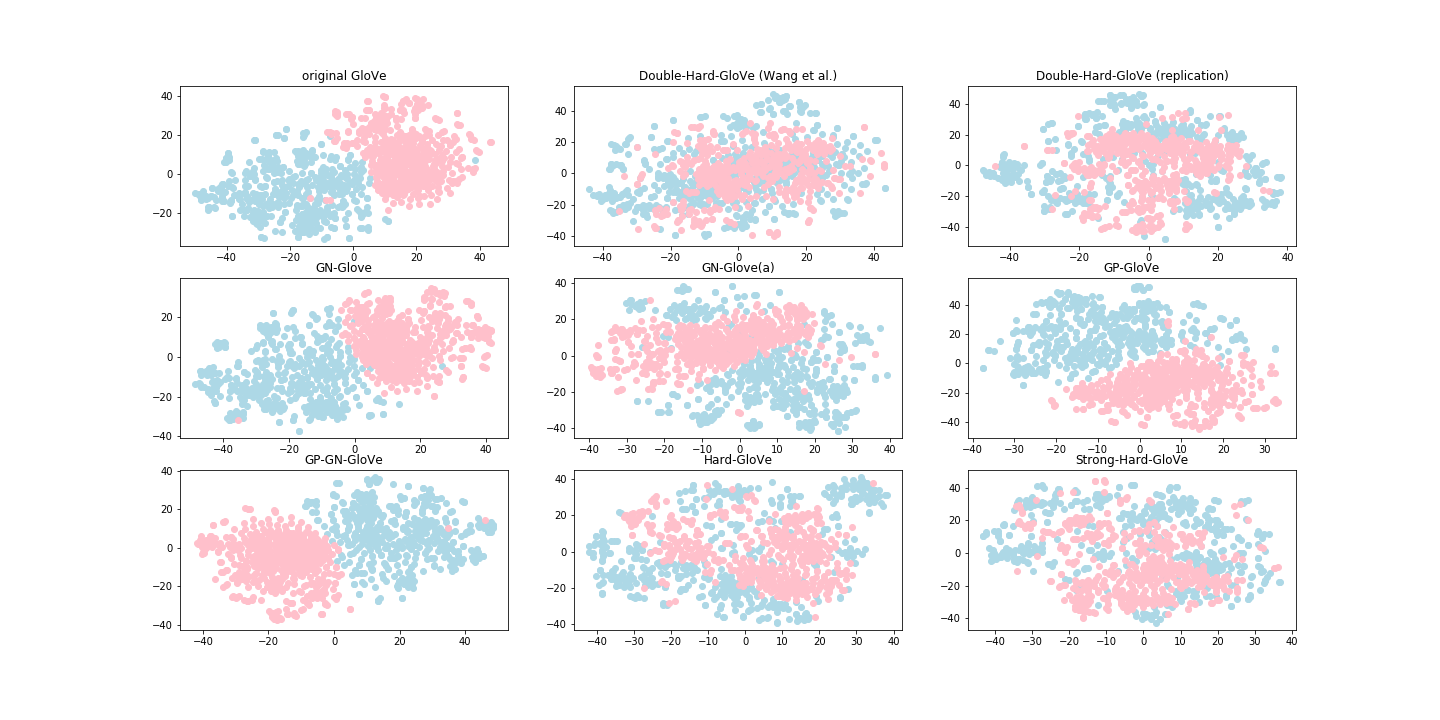
\includegraphics{evaluation_results/results_tsne.png}

\hypertarget{analysis-of-retaining-word-semantics}{%
\subsubsection{Analysis of Retaining Word Semantics}\label{analysis-of-retaining-word-semantics}}

One of the most important properties of embeddings is that they represent meaningful word semantics, for example in the form of analogies or concepts. In this section it is tested in how far the embeddings still meet this criterion after debiasing.

\hypertarget{word-analogy-kristina}{%
\paragraph{Word Analogy (Kristina)}\label{word-analogy-kristina}}

The word analogy task was introduced by Mikolov, Yih, and Zweig (2013). The task is to find the word D such that ``A is to B as C is to D.'' One example for an unbiased analogy is: ``Man is to King as Woman is to Queen'' whereas a biased analogy would be: ``Man is to Computer Programmer as Woman is to Homemaker'' (Bolukbasi, Chang, Zou, Saligrama, \& Kalai, 2016). The debiased embeddings are evaluated on two word analogy test sets, the MSR (Mikolov, Yih, \& Zweig, 2013) and the Google word analogy task (Mikolov, Chen, Corrado, \& Dean, 2013), in order to find out whether they preserve desired unbiased analogies.

The MSR word analogy dataset contains 8000 syntactic questions in the form presented above. The missing word D is computed by maximizing the cosine similarity between D and C - A + B. The evaluation metric is the percentage of correctly answered questions (see Wang et al., 2020).

The Google word analogy dataset contains 19.544 (\textbf{Total}) questions, 8.869 of which are semantic (\textbf{Sem}) and 10.675 are syntactic (\textbf{Syn}) questions.

\begin{table}[tbp]

\begin{center}
\begin{threeparttable}

\caption{\label{tab:table 3}Analogy Tasks}

\begin{tabular}{lllll}
\toprule
Embeddings & MSR & Sem & Syn & Total\\
\midrule
original GloVe & 54.40 & 80.14 & 55.69 & 63.90\\
Double-Hard-GloVe (Wang et al.) & 42.40 & 71.36 & 47.99 & 56.67\\
Double-Hard-GloVe (replication) & 62.12 & 80.20 & 66.55 & 71.13\\
GN-Glove & 51.72 & 75.97 & 54.67 & 61.82\\
GN-Glove(a) & 50.72 & 75.89 & 54.26 & 61.52\\
GP-GloVe & 51.62 & 81.92 & 55.42 & 64.32\\
GP-GN-GloVe & 51.99 & 75.75 & 56.68 & 63.08\\
Hard-GloVe & 62.57 & 80.00 & 66.10 & 70.76\\
Strong-Hard-GloVe & 62.14 & 76.74 & 65.73 & 69.43\\
\bottomrule
\end{tabular}

\end{threeparttable}
\end{center}

\end{table}

The results can be inspected in Table 3 and are in line with the results reported by Wang et al. (2020). What is interesting is that our replicated Double-Hard debiased embedding scores best in all word analogy tasks and even outperforms the original GloVe embedding.

\hypertarget{concept-categorization}{%
\paragraph{Concept Categorization}\label{concept-categorization}}

Wang et al. (2020) applied this evaluation method to all the different embedding baselines and their Double-Hard debiased embedding as well. However, we found the code provided by the authors to be incomplete. It was missing major parts and due to time constraints we decided not to implement this method.

\hypertarget{discussion}{%
\subsection{Discussion}\label{discussion}}

\begin{itemize}
\tightlist
\item
  analysis of results and evaluation of performance evaluation
\item
  ablation studies (not applicable)
\item
  discuss the results and what could be (partly) replicated and what not
\end{itemize}

\hypertarget{conclusion}{%
\subsection{Conclusion}\label{conclusion}}

\newpage

\hypertarget{references}{%
\section{References}\label{references}}

\begingroup
\setlength{\parindent}{-0.5in}
\setlength{\leftskip}{0.5in}

\hypertarget{refs}{}
\begin{CSLReferences}{1}{0}
\leavevmode\hypertarget{ref-baker_2015}{}%
Baker, M. (2015). Reproducibility crisis: Blame it on the antibodies. \emph{Nature}, \emph{521}(7552), 274--276. https://doi.org/\url{https://doi.org/10.1038/521274a}

\leavevmode\hypertarget{ref-belz_2021}{}%
Belz, A., Agarwal, S., Shimorina, A., \& Reiter, E. (2021). \emph{A systematic review of reproducibility research in natural language processing}. Retrieved from \url{http://arxiv.org/abs/2103.07929}

\leavevmode\hypertarget{ref-bolukbasi_2016}{}%
Bolukbasi, T., Chang, K.-W., Zou, J. Y., Saligrama, V., \& Kalai, A. (2016). Man is to computer programmer as woman is to homemaker? Debiasing word embeddings. \emph{CoRR}, \emph{abs/1607.06520}. Retrieved from \url{http://arxiv.org/abs/1607.06520}

\leavevmode\hypertarget{ref-caliskan_2017}{}%
Caliskan, A., Bryson, J. J., \& Narayanan, A. (2017). Semantics derived automatically from language corpora contain human-like biases. \emph{Science}, \emph{356}(6334), 183--186. \url{https://doi.org/10.1126/science.aal4230}

\leavevmode\hypertarget{ref-cohen_2018}{}%
Cohen, K. B., Xia, J., Zweigenbaum, P., Callahan, T., Hargraves, O., Goss, F., \ldots{} Hunter, L. E. (2018). Three dimensions of reproducibility in natural language processing. \emph{Proceedings of the eleventh international conference on language resources and evaluation ({LREC} 2018)}. Miyazaki, Japan: European Language Resources Association (ELRA). Retrieved from \url{https://www.aclweb.org/anthology/L18-1025}

\leavevmode\hypertarget{ref-collberg_2015}{}%
Collberg, C., Proebsting, T., \& Warren, A. M. (2015). \emph{Repeatability and benefaction in computer systems research}. studie. Retrieved from \url{http://reproducibility.cs.arizona.edu/v2/RepeatabilityTR.pdf}

\leavevmode\hypertarget{ref-fokkens_2013}{}%
Fokkens, A., Erp, M. van, Postma, M., Pedersen, T., Vossen, P., \& Freire, N. (2013). Offspring from reproduction problems: What replication failure teaches us. \emph{Proceedings of the 51st annual meeting of the association for computational linguistics (volume 1: Long papers)}, 1691--1701. Sofia, Bulgaria: Association for Computational Linguistics. Retrieved from \url{https://www.aclweb.org/anthology/P13-1166}

\leavevmode\hypertarget{ref-gonen_2019}{}%
Gonen, H., \& Goldberg, Y. (2019). \emph{Lipstick on a pig: Debiasing methods cover up systematic gender biases in word embeddings but do not remove them}. Retrieved from \url{http://arxiv.org/abs/1903.03862}

\leavevmode\hypertarget{ref-gong_2018}{}%
Gong, C., He, D., Tan, X., Qin, T., Wang, L., \& Liu, T.-Y. (2018). FRAGE: Frequency-agnostic word representation. In S. Bengio, H. Wallach, H. Larochelle, K. Grauman, N. Cesa-Bianchi, \& R. Garnett (Eds.), \emph{Advances in neural information processing systems} (Vol. 31, p. ). Curran Associates, Inc. Retrieved from \url{https://proceedings.neurips.cc/paper/2018/file/e555ebe0ce426f7f9b2bef0706315e0c-Paper.pdf}

\leavevmode\hypertarget{ref-greenwald_1998}{}%
Greenwald, A. G., McGhee, D. E., \& Schwartz, J. L. K. (1998). Measuring individual differences in implicit cognition: The implicit association test. \emph{Journal of Personality and Social Psychology}, \emph{74}(6), 1464--1480. \url{https://doi.org/10.1037/0022-3514.74.6.1464}

\leavevmode\hypertarget{ref-kaneko_2019}{}%
Kaneko, M., \& Bollegala, D. (2019). Gender-preserving debiasing for pre-trained word embeddings. \emph{Proceedings of the 57th annual meeting of the association for computational linguistics}, 1641--1650. Florence, Italy: Association for Computational Linguistics. \url{https://doi.org/10.18653/v1/P19-1160}

\leavevmode\hypertarget{ref-mieskes_2017}{}%
Mieskes, M. (2017). A quantitative study of data in the {NLP} community. \emph{Proceedings of the first {ACL} workshop on ethics in natural language processing}, 23--29. Valencia, Spain: Association for Computational Linguistics. \url{https://doi.org/10.18653/v1/W17-1603}

\leavevmode\hypertarget{ref-mieskes_2019}{}%
Mieskes, M., Fort, K., Névéol, A., Grouin, C., \& Cohen, K. B. (2019). {NLP Community Perspectives on Replicability.} \emph{{Recent Advances in Natural Language Processing}}. Varna, Bulgaria. Retrieved from \url{https://hal.archives-ouvertes.fr/hal-02282794}

\leavevmode\hypertarget{ref-mikolov2013Google}{}%
Mikolov, T., Chen, K., Corrado, G., \& Dean, J. (2013). \emph{Efficient estimation of word representations in vector space}. Retrieved from \url{http://arxiv.org/abs/1301.3781}

\leavevmode\hypertarget{ref-mikolov2013MSR}{}%
Mikolov, T., Yih, W., \& Zweig, G. (2013). Linguistic regularities in continuous space word representations. \emph{Proceedings of the 2013 conference of the north {A}merican chapter of the association for computational linguistics: Human language technologies}, 746--751. Atlanta, Georgia: Association for Computational Linguistics. Retrieved from \url{https://www.aclweb.org/anthology/N13-1090}

\leavevmode\hypertarget{ref-mu_2018}{}%
Mu, J., Bhat, S., \& Viswanath, P. (2018). \emph{All-but-the-top: Simple and effective postprocessing for word representations}. Retrieved from \url{http://arxiv.org/abs/1702.01417}

\leavevmode\hypertarget{ref-vaswani_2017}{}%
Vaswani, A., Shazeer, N., Parmar, N., Uszkoreit, J., Jones, L., Gomez, A. N., \ldots{} Polosukhin, I. (2017). \emph{Attention is all you need}. Retrieved from \url{http://arxiv.org/abs/1706.03762}

\leavevmode\hypertarget{ref-wang_2020}{}%
Wang, T., Lin, X. V., Rajani, N. F., McCann, B., Ordonez, V., \& Xiong, C. (2020). Double-hard debias: Tailoring word embeddings for gender bias mitigation. \emph{Association for computational linguistics (ACL)}.

\leavevmode\hypertarget{ref-zhao_2018a}{}%
Zhao, J., Wang, T., Yatskar, M., Ordonez, V., \& Chang, K.-W. (2018, January). \emph{Gender bias in coreference resolution: Evaluation and debiasing methods}. 15--20. \url{https://doi.org/10.18653/v1/N18-2003}

\leavevmode\hypertarget{ref-zhao_2018b}{}%
Zhao, J., Zhou, Y., Li, Z., Wang, W., \& Chang, K.-W. (2018). Learning gender-neutral word embeddings. \emph{Proceedings of the 2018 conference on empirical methods in natural language processing}, 4847--4853. Brussels, Belgium: Association for Computational Linguistics. \url{https://doi.org/10.18653/v1/D18-1521}

\end{CSLReferences}

\endgroup


\end{document}
